\section*{Cara pakai kondisi didalam kondisi}

\par
Didalam python kita dapat melakukan logika kondisi didalam kondisi. caranya sebagai berikut


 \begin{enumerate}
	\item buka aplikasi spyder lalu tuliskan codingan dengan logika dan kondisi sebagai berikut
	\begin{figure} [h]
	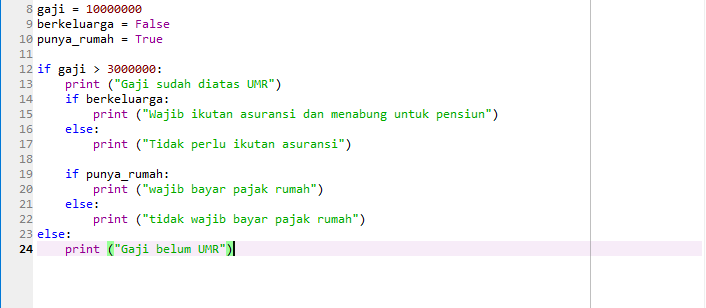
\includegraphics[width=9cm]{if/if1.png}
	\centering
	\end{figure}
	
	 
	\item kalian bisa memilih kondisi yang kalian inginkan. bisa False bisa True. dan mengisi jumlah gaji sesuai keinginan kalian
	
	\item Maka output akan seperti berikut
	\begin{figure} [h]
	
\includegraphics[width=10cm]{if/if2.png}
	\centering
	\end{figure}
	
	
	
	
	
    \end{enumerate}



